\begin{surferIntroPage}{Tutorial}{tutorial_koord1}{Primi passi con SURFER}
Questo programma si chiama SURFER. Leggendo il nome penserai forse al mare,  al sole e alle onde. Invece in questo caso il nome viene dalla parola inglese {\it surface} che vuol dire {\it superficie}.
\\
Con SURFER puoi creare superfici, pi\`u precisamente superfici algebriche. Cosa siano le superfici algebriche e come funzioni il programma viene spiegato in questo tutorial. Scegli una delle superfici sulla destra per leggere il corrispondente capitolo del tutorial.\\
SURFER fa parte della mostra itinerante IMAGINARY che \`e nata nell'Anno della Matematica 2008, in Germania. La mostra \`e un progetto del centro di ricerca internazionale ``Mathematisches Forschungsinstitut Oberwolfach", situato nella Foresta Nera.  Presso l'istituto  si tengono ogni settimana conferenze su argomenti attuali di ricerca in matematica. Questi incontri sono molto importanti perch\'e permettono a scienziati di tutto il mondo di scambiarsi le loro conoscenze.\\
\vspace{0.2cm} \hspace{3.5cm}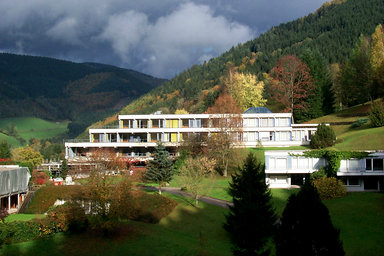
\includegraphics[width=3cm]{./../../common/images/photo_mfo.jpg}\\
Il programma SURFER pu\`o essere scaricato gratuitamente dalla nostra homepage:\\
\begin{centering}
www.imaginary.org\\
\end{centering}
 \vspace{0.2cm}
A destra puoi scegliere uno dei tutorial matematici, che iniziano con la superficie Limone. A sinistra puoi invece andare alle altre gallerie, per esempio alla galleria delle superfici fantastiche.
\end{surferIntroPage}


